
\renewcommand{\EntradaBibtex}{ClasificadorHabaneros_ProcesadoresDigitales_UPV_2023}


\begin{frame}{\citetitle{\EntradaBibtex}$^*$ (1)}
\begin{block}{Propuesta} 
Una aplicación que clasifique chiles habaneros por su grado de madurez
\end{block} 
\begin{itemize}
\item Se creó un dataset con 3 niveles de madurez (verde, amarillo y rojo) y un nivel ``No-Chile''
\item Se codificó una aplicación que permite al usuario seleccionar regiones rectangulares de una imagen y asignarles el nivel de madurez de manera manual
\item Se entrenaron diferentes modelos para obtener el de mejor desempeño
\item La idea a futuro es integrar este clasificador con un sistema hidropónico para monitorear de manera remota un cultivo y establecer el tiempo de cosecha optimo de cada chile.
\end{itemize}
\footfullcite*{\EntradaBibtex}
\end{frame}

\begin{frame}{\citetitle{\EntradaBibtex} (2)}

\begin{center}
	\begin{tabular}{ccc}
		\includegraphics[width=0.20\linewidth]{2023_ChilesHabaneros/figs/im1.png} &
		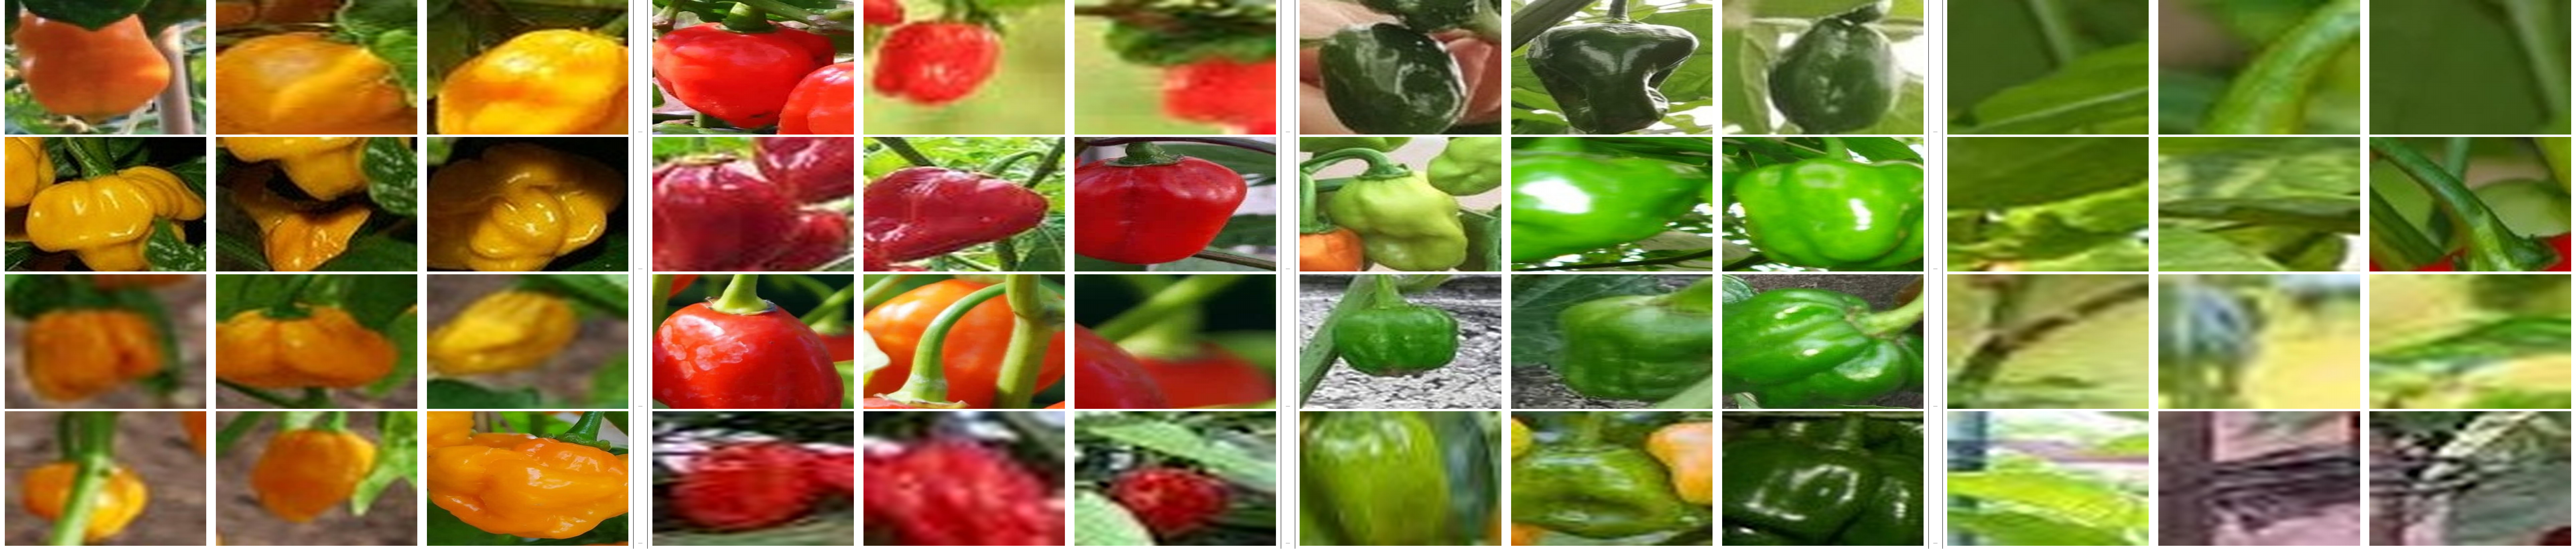
\includegraphics[width=0.75\linewidth]{2023_ChilesHabaneros/figs/Mosaico.png} & \\
	\end{tabular}
\end{center}

\end{frame}

%


